%%%%%%%%%%%%%%%%%%%%%%% file template.tex %%%%%%%%%%%%%%%%%%%%%%%%%
%
% This is a general template file for the LaTeX package SVJour3
% for Springer journals.          Springer Heidelberg 2010/09/16
%
% Copy it to a new file with a new name and use it as the basis
% for your article. Delete % signs as needed.
%
% This template includes a few options for different layouts and
% content for various journals. Please consult a previous issue of
% your journal as needed.
%
%%%%%%%%%%%%%%%%%%%%%%%%%%%%%%%%%%%%%%%%%%%%%%%%%%%%%%%%%%%%%%%%%%%
%
\RequirePackage{fix-cm}
%
%\documentclass{svjour3}                     % onecolumn (standard format)
%\documentclass[smallcondensed]{svjour3}     % onecolumn (ditto)
\documentclass[smallextended]{svjour3}       % onecolumn (second format)
%\documentclass[twocolumn]{svjour3}          % twocolumn
%
\smartqed  % flush right qed marks, e.g. at end of proof
%
\usepackage{graphicx}
%
% \usepackage{mathptmx}      % use Times fonts if available on your TeX system
%
% insert here the call for the packages your document requires
\usepackage[square,numbers,comma]{natbib}
\usepackage{amssymb}
\usepackage{amsmath}
\usepackage{url}
\usepackage{array}
\usepackage[ruled,lined,vlined]{algorithm2e}
% etc.
%
% please place your own definitions here and don't use \def but
% \newcommand{}{}
%
% Insert the name of "your journal" with
\journalname{The Journal of Supercomputing}
%
\begin{document}

\title{PARIS: A PArallel RSA-prime InSpection tool%\thanks{Grants or other notes
%about the article that should go on the front page should be
%placed here. General acknowledgments should be placed at the end of the article.}
}
%\subtitle{Do you have a subtitle?\\ If so, write it here}

%\titlerunning{Short form of title}        % if too long for running head

\author{Joseph White\and
        Christopher Lupo%etc.
}

%\authorrunning{Short form of author list} % if too long for running head

\institute{J. White \and C. Lupo\at
              California Polytechnic State University
              1 Grand Ave, San Luis Obispo, CA 93407\\
              Tel.: +805-756-5659\\
              \email{\{jwhite09, clupo\}@calpoly.edu}           %  \\
%             \emph{Present address:} of F. Author  %  if needed
}

\date{Received: date / Accepted: date}
% The correct dates will be entered by the editor


\maketitle

\begin{abstract}
Modern-day computer security relies heavily on cryptography as a means to
protect the data that we have become increasingly reliant on. As the Internet
becomes more ubiquitous, methods of security must be better than ever.
Validation tools can be leveraged to help increase our confidence and
accountability for methods we employ to secure our systems. 

Security validation, however, can be difficult and time-consuming. As our
computational ability increases, calculations that were once considered ``hard"
due to length of computation, can now be done in minutes. We are constantly
increasing the size of our keys and attempting to make computations harder to
protect our information. This increase in ``cracking" difficulty often has the
unfortunate side-effect of making validation equally as difficult.

We can leverage massive-parallelism and the computational power that is granted
by today's commodity hardware such as GPUs to make checks that would
otherwise be impossible to perform, attainable. Our work presents a practical
tool for validating RSA keys for poor prime numbers: a fundamental problem
that has led to significant security holes, despite the RSA algorithm's
mathematical soundness.

Our tool, PARIS, leverages NVIDIA's CUDA framework to perform a complete set of
greatest common divisor calculations between all keys in a provided set. Our
implementation offers a 27.5 times speedup using a GTX 480 and 33.9 times
speedup using a Tesla K20Xm: both compared to a reference sequential
implementation for sets of less than 200000 keys. This level of speedup brings
this validation into the realm of practicality due to decreased runtime.

\keywords{CUDA \and RSA \and greatest common divisor \and parallel computation}
\end{abstract}

%%%%%%%%%%%%%%%%%%%%%%%%%%%%%%%%%%%%%%%%%%%%%%%%%%%%%%%%%%%%%%%%%%%%%%%%%%%%%%%%

\section{Introduction}
\label{sec:intro}
RSA (named for its inventors, Ron Rivest, Adi Shamir, and Leonard Adleman) is a
public key encryption scheme which relies on the difficulty of factoring large
numbers. The algorithm is prevalent throughout security, and is specifically
used for many web-security applications (see $\S$\ref{sec:motivation}). An RSA
key contains public and private components, both of which are calculated based
on two randomly-generated prime values: $p$ and $q$ (RSA is explained at
greater length in $\S$\ref{subsec:rsa}). Ideally, given the number of possible
primes that may be used to construct a 1024-bit key, no random number
generators should reuse either prime, and all keys should contain unique
components. Thus, the likelihood of either $p$ or $q$ being repeated in a set
of keys should be approximately 0. Since in reality, random number generation
is difficult, and often less than random, primes are, in fact, repeated. Due to
this, an individual key may be considered secure by itself, but when compared
to other keys might exhibit a weakness which allows each key's private
components to be calculated entirely from public information.  

When considering two keys, a weakness exists when the \textit{greatest common 
divisor} (GCD) of both moduli, $n_1$ and $n_2$, is greater than 1. If $GCD(n_1, 
n_2) = p$, then $p$ must be a shared prime factor of $n_1$ and $n_2$. Thus, 
$q_1 = \frac{n_1}{p}$ and $q_2 = \frac{n_2}{p}$. Once $p$ and $q$ are known,
$d_1$ and $d_2$ (values in the private components) can be directly calculated,
yielding both private key pairs. This vulnerability is detailed in
Figure~\ref{fig:vuln}.

This weakness is discussed in \cite{lenstra2012ron}, which shows a significant
number of existing RSA keys were susceptible to this exploit. The primary goal
of our work was to speedup the most computationally intensive part of their
process by implementing the GCD comparisons of RSA 1024-bit keys using NVIDIA's
CUDA platform.

To aid in accomplishing this goal, the work in \cite{fujimoto2009high} was 
expanded and adapted to compare all combinations of keys in a given set. In 
comparison to their work, larger sections of the overall program were able to 
be executed in parallel, resulting in further speedup. We implemented this in a
recent paper and applied it to sets of RSA moduli. While successful, this work
(\cite{scharfglass2012breaking}) was only capable of validating a single set of
keys whose size was constrained by the GPU memory. In our new work here, we
focus on overcoming this limitation, and add the ability to process sets of
keys of arbitrary length.

\subsection{The Meaning of PARIS}
\label{subsec:meaning}

The title of our validation tool has meaning beyond its descriptive acronym,
and contains ties to Greek Mythology. The Greek hero Achilles was known for
his greatness and is the central character of many Greek myths including
Homer's epic, \textit{The Iliad}\cite{homer2009iliad}. He is probably best
known for his single fatal weakness: his heel. According to myth, his body was
made invulnerable at birth by being dipped into the river Styx. This
invulnerability made him the great warrior that he was; however, his mother
held him by his heel as she dipped him into the river, leaving it exposed and
thus vulnerable. This marks his weakness, and after a short life filled with
battle and warfare, a fatal arrow wound through his heel results in his death.

We look to this myth as an analogy for the RSA algorithm. RSA can be viewed as
Achilles: a character with epic strength (i.e. mathematical soundness) capable
of feats never before possible (i.e. cryptographic communications).
However, it has a single, fatal flaw: random prime numbers. This weakness, for
Achilles, was exposed by an arrow shot by Paris, Prince of Troy. It is here,
that we derive our tool's name.

We use Paris because he exposed the weakness in a great hero. In the same way,
we aim to make finding the flaw of poor random number generation in RSA keys
a more public and accessible task. 

%%%%%%%%%%%%%%%%%%%%%%%%%%%%%%%%%%%%%%%%%%%%%%%%%%%%%%%%%%%%%%%%%%%%%%%%%%%%%%%%

\section{Background}
\label{sec:background}

\subsection{RSA}
\label{subsec:rsa}
RSA is an asymmetric key encryption scheme. Keys come in matched pairs: a
public key and a private key. The public key is comprised of a modulus $n$ of
specified length (the product of primes $p$ and $q$), and an exponent $e$. The
length of $n$ is given in terms of bits, thus the term ``1024-bit RSA key"
refers to the number of bits which make up this value. The associated private
key uses the same $n$, and another value $d$ such that $d \cdot e = 1
\:\text{mod} \;\phi(n)$ where $\phi(n) = (p - 1) \cdot (q - 1)$
\citep{rivest1978method}.

Using the same algorithm, information encrypted with the one key can be
decrypted with the other and vice versa. A party must keep the private key
secret, but the public portion of the key can be seen and used by anyone in the
world. To generate a public-private key pair, an algorithm is implemented using
two randomly-generated prime numbers whose product is of a certain bit-length
(e.g. 1024 bits). PARIS aims to uncover the inadequacies present in these
primes.

%The work presented by \cite{lenstra2012ron} shows that around 0.2\% of RSA keys
%collected from sources including the SSL Observatory suffer from inadequate
%random prime generation. They show that when the primes used to build an RSA
%public-private key pair are not actually random, factoring does not need to be
%done to break the keys. Instead, only a greater common divisor needs to be
%calculated between two RSA moduli. When anything greater than 1 is found as a
%result of this calculation, the keys can be considered broken and offer no
%protection. This is because once a GCD greater than 1 is found, the private
%keys can be generated from the publicly available information. The
%vulnerability is explained in detail in Figure~\ref{fig:vuln}.

\begin{figure}
   \centering
   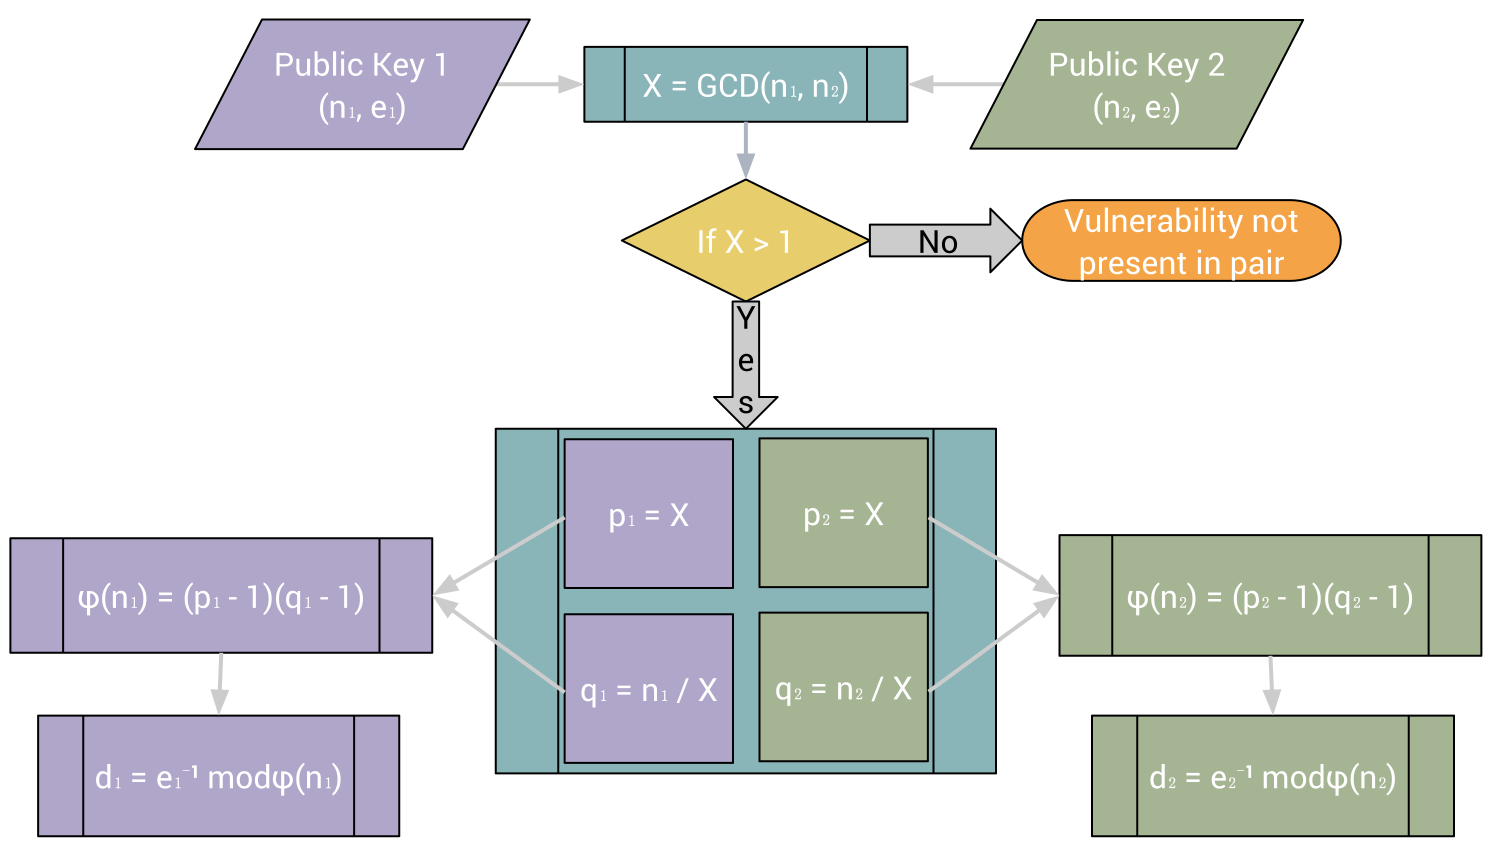
\includegraphics[width=\textwidth]{vulnerability}
   \caption{Explanation of poor-prime vulnerability}
   \label{fig:vuln}
\end{figure}

%A tool by \cite{scharfglass2012breaking} performs a
%parallelized version of this GCD calculation (using the binary GCD algorithm)
%between every pair combination in a given set of keys. It structures these
%calculations so that as many as possible can be done at once. To increase
%parallelism, and because the keys are so large, they are broken up into 32
%chunks, which are also operated on in parallel using the GPU. Through these 2
%levels of parallelism, a speedup of 27.5 is achieved. This tool provides a
%practical tool for checking a given set of keys for the vulnerability we are
%focusing on.

\subsection{CUDA}
\label{subsec:cuda}
NVIDIA's \textit{Compute Unified Device Architecture} (CUDA) is a platform that
provides a set of tools along with the ability to write programs that make use
of NVIDIA's GPUs (cf.  \cite{nvidia2012programming}). These massively-parallel
hardware devices are capable of processing large amounts of data
simultaneously, allowing significant speedups in programs with sections of
parallelizable code using the Simultaneous Program, Multiple Data (SPMD)
model. The platform allows for various arrangements of threads to perform work,
based on the developer's decomposition of the problem. Our solution is
discussed in $\S$\ref{subsec:gridorg}. In general, individual threads are grouped
into up-to 3-dimensional blocks to allow sharing of common memory between
threads. These blocks can then be organized into a 2-dimensional grid.  

The GPU breaks the total number of threads into groups called warps, which, on
current GPU hardware, consist of 32 threads that will be executed
simultaneously on a single \textit{streaming multiprocessor} (SM). The GPU
consists of several SMs which are each capable of executing a warp. Blocks are
scheduled to SMs until all allocated threads have been executed. 

There is also a memory hierarchy on the GPU. Three of the various types of
memory are relevant to this work: global memory is the slowest and largest;
shared memory is much faster, but also significantly smaller; and a limited
number of registers that each SM has access to. Each thread in a block can
access the same section of shared memory.

%%%%%%%%%%%%%%%%%%%%%%%%%%%%%%%%%%%%%%%%%%%%%%%%%%%%%%%%%%%%%%%%%%%%%%%%%%%%%%%%

\section{Motivation}
\label{sec:motivation}
Despite PARIS's focus on performance and speedup of the vulnerability check,
its impacts and implications to computer security are equally important.
We look into some of RSA's more popular applications to help motivate why our
work and PARIS's increase in practicality is important to the world of computer
security. We aim to discuss what types of data might be vulnerable due to this
exploit (as well as others affecting RSA), impacts the vulnerability has, and
put a portion of the current state of computer security into a real-world
context concerning RSA.

Most initial research yielded general statements that did not explain or give
appropriate context to RSA (statements including ``\dots all over the
Internet\dots" were accurate, but not informative). More in-depth research
yielded two primary use-cases of RSA: Digital Rights Management (DRM) and
Secure Socket Layer (SSL) / Transport Layer Security (TLS) Internet
security protocols. Other uses included password alternatives (e.g. ssh
connections or command line interface tools like \texttt{git}) but these are
more difficult to collect data for and analyze since they tend to be done on
an individual basis, and are managed by individual users.

\subsection{Digital Rights Management}
\label{subsec:drm}
Digital rights management is a protocol used to secure the usage and
distribution of various types of media content. It is adopted by content
providers and device manufacturers to ensure users don't misuse or wrongfully 
share protected, copyrighted content. The RSA Association proposed a protocol
that could be applied to various types of media content that secured its usage
\citep{rsa2004announces,rsa2004supports}. These announcements argued that using
RSA for DRM offered benefits to the content providers, the device
manufacturers, and, arguably, the consumers of the content. It allows device
manufactures and content providers to ensure proper usage of protected content
while allowing users to consume and playback their rightfully-owned media on an
array of their own devices.

\subsection{Internet Security and Certificates}
\label{subsec:netsec}
Internet security relies on a particular protocol called SSL and its successor
TLS. These protocols define how to securely transfer information over the
Internet by using encryption and signing mechanisms. One aspect of both the SSL
and TLS protocols involve certificates to ensure the expected party is
actually being communicated with. These certificates provide information
about a server that a user is connected to (e.g. Amazon or Google)
and is signed by a certificate authority (e.g. VeriSign). These certificates
are also encrypted with a subject's (e.g. Amazon) public key to ensure that
the entity is who they say they are. Furthermore, the public key is then used 
to transfer information back to the subject in a secure way.
Figure~\ref{fig:tls} describes the TLS process between a client and server. 

The most widely used type of certificate is the X.509 certificate, whose current
revision is 3. A breakdown of the major sections of the certificate is shown in
Figure~\ref{fig:x509}. The ``Subject Public Key Information" section of the
certificate holds the relevant data (the subject's RSA public key) for our work.
The public key portion of the certificates can actually use one of several
algorithms defined in the specification. RSA is by far the most popular,
accounting for over half of the found certificates (as shown in
Figure~\ref{fig:certs}). Other options include DSA and Diffie-Hellman. For more
detailed information about X.509 certificates and analysis on their
infrastructure, see \citet{holz2011ssl}.

\begin{figure}
   \centering
   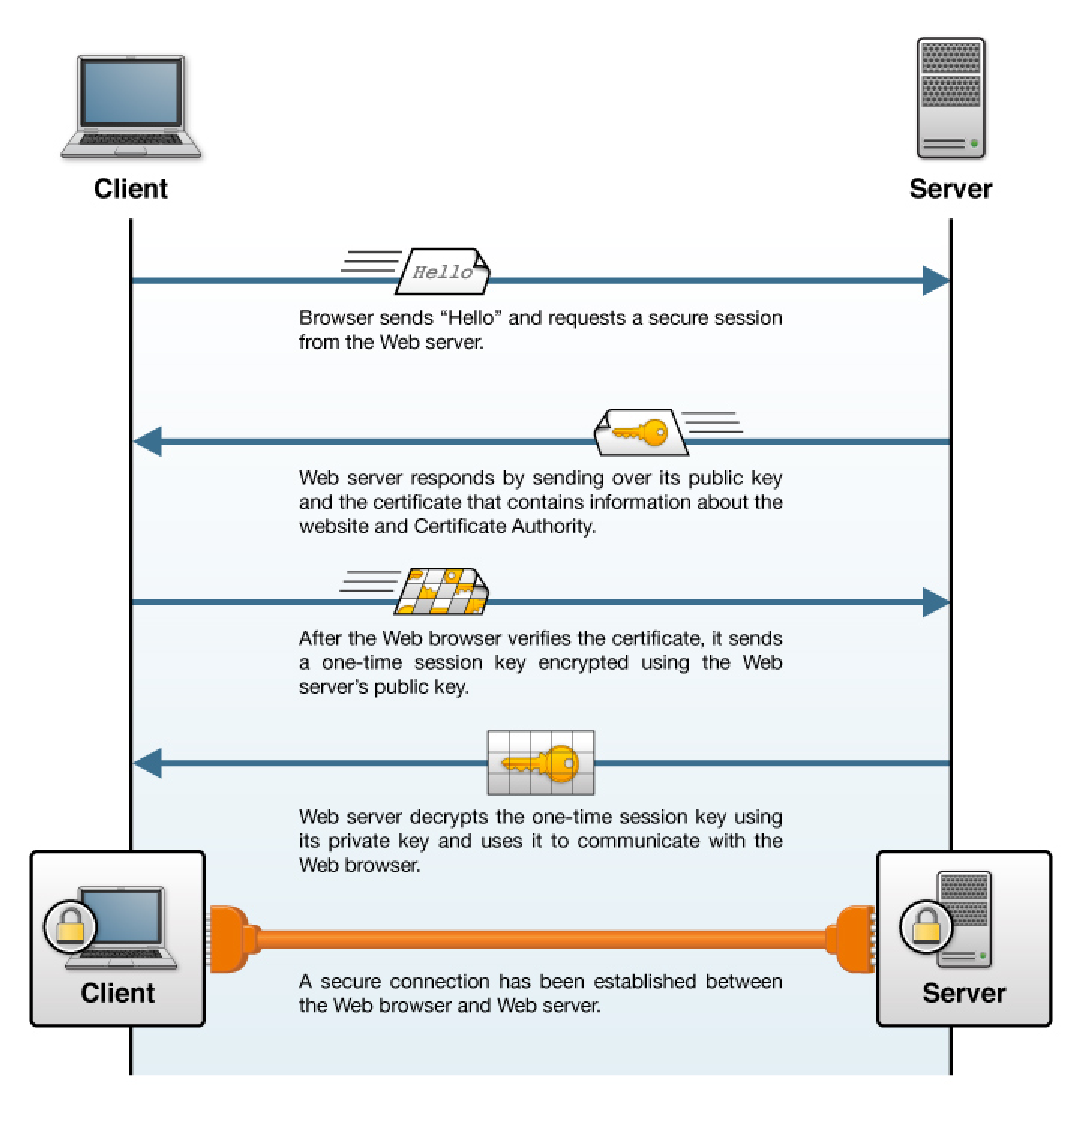
\includegraphics[width=0.75\textwidth]{tls}
   \caption{TLS Overview \citep{tlsconcepts}\label{fig:tls}}
\end{figure}

\begin{figure}
   \centering
   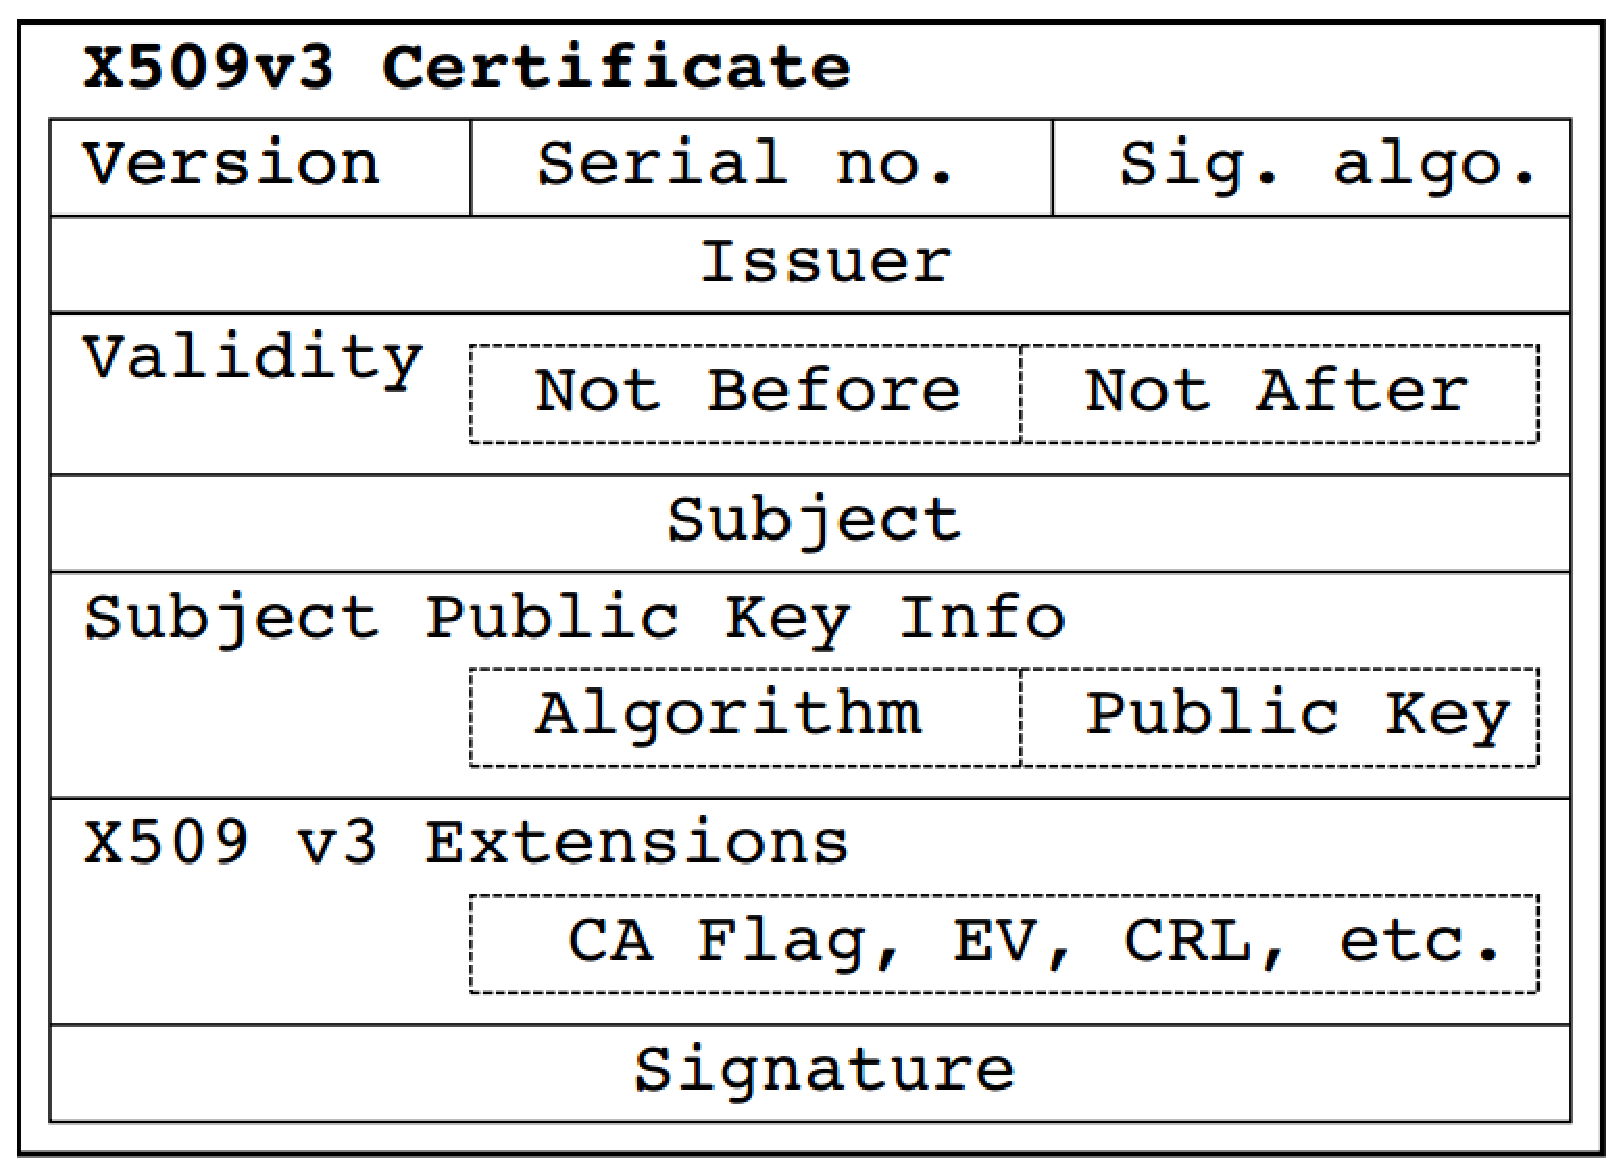
\includegraphics[width=0.75\textwidth]{x509}
   \caption{X.509 Fields \citep{holz2011ssl}\label{fig:x509}}
\end{figure}

\subsection{Data Collection}
\label{subsec:datacol}
The proposed DRM protocol given by the RSA Association closely follows the
certificate model used by SSL/TLS. For this reason, the SSL certificate model
was the primary focus of the data collected. Moreover, the data set of RSA keys
in SSL certificates is much larger than DRM implementations that use RSA. Thus,
the data set that was collected and then analyzed consisted entirely of X.509
certificates.

Since a primary motivation of this work is the potential impact that vulnerable
RSA keys may have, a data set representative of a large portion of traffic was
desired. A survey was done over 2007-2010 \citep{labovitz2011internet} that
gathered some useful data on the Internet as a whole. Relevant to web traffic,
this study showed that together, the major \textit{content data networks }(CDN)
(i.e. Google, Facebook, Amazon, etc.) account for nearly 17\% of web traffic. 
Specific breakdowns and conversions can be found in Table~\ref{tab:traffic}.

\begin{table}
\centering
\caption{Major CDN Traffic (2010)}
\begin{tabular}{|>{\raggedright}p{0.4\linewidth}
                |>{\raggedright}p{0.2\linewidth}
                |>{\raggedright\arraybackslash}p{0.2\linewidth}|}\hline
   \textbf{CDN} & \textbf{Percent of all Internet traffic} & \textbf{Approx. percentage of web traffic}\\ \hline
Google & 7 & 12.72\\ \hline
LeaseWeb (Heineken, Starbucks,\dots) & 0.8 & 1.454\\ \hline
Amazon CDN (NASA/JPL, PBS,\dots) & 0.55 & 1\\ \hline
EdgeCast (Yahoo!, Break, Imgur,\dots) & 0.5 & 0.909\\ \hline
Facebook & 0.45& 0.818\\
\hline\end{tabular}
\label{tab:traffic}
\end{table}

Alexa was used to find websites with large amounts of
traffic\footnote{http://www.alexa.com/}, as it serves as one of the Internet's
most prevalent sources for traffic information. In addition to individualized
site traffic data, Alexa provides a daily-updated list of the top one million
websites ordered by
traffic\footnote{http://s3.amazonaws.com/alexa-static/top-1m.csv.zip}. In
regards to the previous point concerning CDNs and traffic breakdowns, it was
noted that all web sites hosted by the major CDNs from
\cite{labovitz2011internet} are present in the top one million list.
Additionally, the vast majority of sites from the top one million list were
not provided by the CDNs mentioned in \cite{labovitz2011internet}. This means
that a much larger percentage than 17\% is actually represented by the sites
in the list, although quantifying precisely how much becomes difficult, and
lies beyond the scope of this project.

A Python script was used to parse the \textit{comma separated value} (CSV) file
provided by Alexa. Each extracted URL was visited on port 443 (corresponding to
``https://") using \texttt{openssl}. If a site responded on that port, it
provided an X.509 certificate to be parsed and verified. During a normal web
session, this is done by a user's web browser which has certificate
authorities' private keys hidden within. However, since the work here was not
concerned with the actual web content, the certificate was simply saved. When
certificates were found, the ``Subject Public Key Algorithm" section was
inspected. If this contained some form of RSA, \texttt{openssl} was used again
to extract the RSA key and save it into a \textit{Privacy Enhanced Mail} (PEM)
file (a standard format for saving public and private key information in).
Additionally, since part the motivation of data collection is PARIS, the keys
were also stored into a SQLite3 database so that later retrieval using PARIS
was trivial.  

Some of Python's
multi-process capabilities were utilized to speed up the collection of data.
Eight processes were spawned to perform the work described above. Seven of the
processes read URLs from a deque (double-ended queue) and attempted to obtain
an X.509 certificate and RSA key from each. When found, these keys were added
to a queue. These data structures not only offered convenient structures for
organizing the data, but were also thread-safe and could be used with our
updated implementation. An eighth thread read keys from the queue and entered
them into the SQLite3 database. This reimplementation offered a 15$\times$
speedup over a single-threaded approach.

\subsection{Data Analysis}
\label{subsec:dataanalysis}
After collecting data from each of the top one million Alexa sites, some
surface-level analysis was performed in order to gain an overview of the
security of these one million sites. This analysis included overall security
breakdowns (i.e. whether a site used any kind of security) and
bit-length breakdowns of the RSA keys that were found. This data analysis can
be found in Figures~\ref{fig:certs} and \ref{fig:bits}. Table~\ref{tab:bits}
shows specific breakdowns for bit-lengths, and offers details that cannot be
seen in the figure.

\begin{figure}
   \centering
   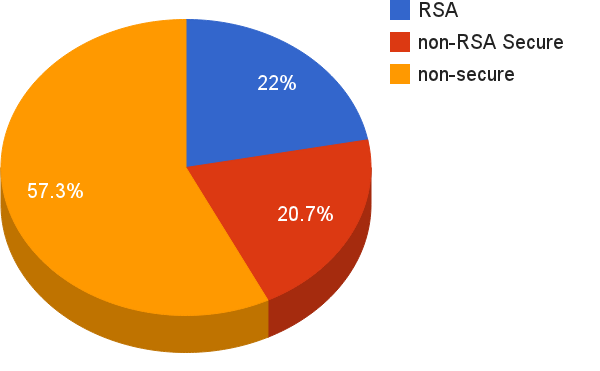
\includegraphics[width=0.75\linewidth]{cert_security}
   \caption{Presence of RSA key or other security in Alexa top 1M sites}
   \label{fig:certs}
\end{figure}

An interesting (and slightly worrisome) observation is that the majority of web
sites in this top one million list did not even respond on port 443, implying
that they do not allow any option for secure traffic to their site. Nearly 60\%
of websites in the list fell into this category.

Also of note are the specifics of bit-lengths found. It is a surprising data
set for various reasons. First, bit-lengths as small as 384, 512, and 768 were
not expected since keys of this size were factored years ago
\citep{rsa2007challenge}, and cannot be expected to offer much
security.

The fact that the majority of keys were 2048-bit was not expected, but means
that a large number of high-traffic websites have adequate (for now)
encryption. Moreover, there were quite a number of sites with 4096, and, even
more surprisingly, 8192-bit.

\begin{figure}
   \centering
   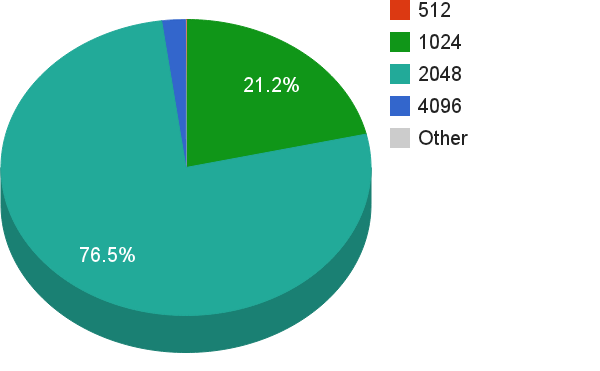
\includegraphics[width=0.75\linewidth]{bit_length}
   \caption{Breakdown of Alexa top 1M sites' RSA keys by bit-length}
   \label{fig:bits}
\end{figure}

\begin{table}
\centering
\caption{Alexa top 1M X.509 RSA bit-length\label{tab:bits}}
\begin{tabular}{|l|r|}\hline
\textbf{Bits} & \textbf{Count}\\\hline
384 & 4 \\ \hline
512 & 309 \\ \hline
768 & 4 \\ \hline
1024 & 46736 \\ \hline
2048 & 168391 \\ \hline
2432 & 37 \\ \hline
3072 & 17 \\ \hline
4096 & 4511 \\ \hline
8192 & 14 \\ \hline
other & 44 \\ \hline
\end{tabular}
\end{table}

Following the surface-level analysis, PARIS was used to perform a complete
check of all RSA keys in a set in order to check for the previously mentioned
vulnerability \citep{lenstra2012ron}. At the time this data was analyzed, PARIS
was limited to 1024-bit RSA keys. Due to this limitation, the data set was
reduced to 46,736 RSA keys. The $O(n^2)$ nature of this problem resulted in
$1,092,150,216$ comparisons. Running PARIS on this data set took 138 minutes,
37 seconds or $131,305$ comparisons per second.  After applying PARIS to this
set of keys, it was found that no keys were susceptible to the vulnerability
(insofar as none of the keys in the set shared primes with any other key in the
set). Although no vulnerabilities were detected, this does not mean the set is
completely secure from the previously mentioned vulnerability. Since such a
limited data set was used, and the security tool relies on large sets to
accumulate many primes, the analysis presented can only be considered an
initial pass.  

\subsection{Implications}
\label{subsec:implications}
For the same reasons the data set was chosen to be X.509 certificates, presence
of the vulnerability mentioned here would have the largest effect on Internet
security: specifically in the certificate infrastructure. If servers were
unknowingly providing compromised public keys in their certificates, their
traffic could offer no security if this became known. This could offer
ill-effects since the vulnerability is agnostic of the type of data being
being encrypted.

Additionally, the password-alternatives that were mentioned briefly before
could be particularly impacted. If a system was generating many new RSA keys
(e.g. a user is building new accounts for various websites, and tying RSA keys
to them) with inadequate primes, potentially all these accounts for this user
could end up compromised, despite the sense of stronger security.

Along these lines, a system administrator could potentially suffer from similar
issues. If many machines and key-pairs are being setup and generated as part of
an initial setup process for a new network of users, poor random number
generation could have severe consequences when done at scale. This would likely
create many new, vulnerable keys at once. By being aware that this problem
could exist, and that a tool such as PARIS exists, an insecure set of keys 
could be avoided or detected much earlier than would have otherwise been
possible.  

%%%%%%%%%%%%%%%%%%%%%%%%%%%%%%%%%%%%%%%%%%%%%%%%%%%%%%%%%%%%%%%%%%%%%%%%%%%%%%%%

\section{Related Works}
\label{sec:related}

\subsection{The Vulnerability}
\label{subsec:vuln}
An RSA vulnerability was discovered and detailed in \cite{lenstra2012ron} in
early 2012 that forms the basis of the exploit the work presented here builds
upon. Namely, that poor random number generation in RSA keys results in
insecure encryption using these keys. Specifically, a key's private components
can be generated using publicly available information.

The exploit explored in \cite{lenstra2012ron} makes use of the two prime
values that play a fundamental role in an RSA key. These values must be
sufficiently random such that repeated values are infeasible and mathematically
extremely improbable to encounter due to the scope of the set (PARIS focuses on
1024-bit keys). However, on some systems and due to some less-than-adequate
code, this may not always be the case. When these values are repeated between
keys, the greatest-common-divisor algorithm can be applied to find the shared
value between keys. This is significant because the GCD calculation is
significantly less computationally expensive than the alternative: factoring
the large values. With this new information about each key, the private
components are straight-forward to generate since the RSA key-generation
process is public and not difficult to implement.  

A large sample set was obtained via the OpenSSL Observatory and by
systematically indexing numerous websites for SSL certificates (which use RSA
as an encryption scheme). Since it was thought this would provide an adequate
sample set, all these keys were analyzed. The set contained 1024-bit keys, as
well as 2048-bit keys. The findings were that 0.2\% of these keys were
vulnerable to this exploit, and thus offered no security. This included
2048-bit keys as well, despite the perception that 2048-bit keys are more
secure (this would be true if this vulnerability were avoided).

Another work that makes extensive mention of this type of vulnerability and the
random prime number problem in general is \cite{heninger2012mining}. Heninger
et al. focus on RSA and DSA and implications poor random number generation can
have. They also used the EFF's release of TLS certificates from the SSL
observatory as their primary data set. Some GCD calculations are done as well,
and they are able to generate various amounts of private keys depending on the
data set.

\subsection{The Process}
\label{subsec:process}
As mentioned, the vulnerability is exploited by performing greatest common
divisor (GCD) calculations with pairs of keys. The research presented here
looks at how to most quickly and efficiently analyze a large database of
RSA keys and detect if this vulnerability is present within the set.
Traditionally, this would be a tedious process that would likely be infeasible
due to time constraints. Since the calculations are independent of one another
(between pairs of keys) they can be done in parallel, given the proper system.
One such system, and the focus of this work, is NVIDIA's CUDA. This will be
detailed later, however, it relates to work done in \cite{fujimoto2009high}. 

Fujimoto's work optimized a specific version of the GCD (binary GCD). This
method reduces the algorithm to three repeated operations. This algorithm was
then implemented in CUDA for 1024-bit numbers (something CUDA does not offer
native support for). This allows much of each operation to be performed in a
parallel fashion, further optimizing the process.

\subsection{Multiple GPUs}
\label{subsec:muliGPU}
%As an extension to the work in \cite{scharfglass2012breaking}, multiple GPU
%support will be explored. This concept is discussed at length in
%\cite{schaa2009exploring}. Here, several GPU configurations are investigated to
%analyze how a distributed system may benefit over a single-GPU design.
%Work is divided intelligently among the systems in the distributed system to
%gain more performance increase than would be possible with a single system.
%
%At the time \cite{schaa2009exploring} was written, single-system,
%multiple-GPU configurations were not possible using CUDA over SLI (Scalable
%Link Interface, NVIDIA's brand for the interface between multiple GPUs).
%However, this is possible now, and will be explored at length in our work.
%This configuration offers benefits including transfer speeds over alternative
%configurations.

The work done in \cite{thibault2009cuda} helps to make a case for the
additional speedup that making use of multiple GPUs can offer. Their work was
done after CUDA had added adequate support for using multiple GPUs
simultaneously, and configurations with two-GPU and four-GPU systems were used.

Significant additional speedups were gained, ranging up to three times speedup
using four GPUs over the single-GPU system (which translates to 100 times
speedup compared to the original, non-GPU benchmark being used). This kind of
speedup offers great optimism in how multiple GPUs may offer significant
increases to performance of the GCD key algorithm.

Another interesting aspect of the work done in \cite{thibault2009cuda} is the
varied domain sizes that were used. The data sets were broken down into several
different configurations which was each tested on the single, dual, or quad-GPU
configuration. This was done to achieve a more accurate answer to how much
faster the multi-GPU system could be. The largest domain set
($1024\times32\times1024$), interestingly, offered the greatest additional
speedup between configurations---the quad-GPU configuration was 3 times faster
than the single-GPU, compared to 2 times for the $256\times32\times256$
domain. This is significant, and implies that exploring different ways to
organize our own data may offer increased advantages when moving to a multi-GPU
system.

\subsection{Large Data}
\label{subsec:largedata}
Wu et al. \cite{wu2009clustering} explore a data set, like our own, where the
data is too large to fit within the limited memory of the GPU. Thus, the data
must be partitioned. In this work, the data was first prepared by organizing it
so that it could be effectively partitioned. There was a straightforward way of
doing so for this application (K-means).  

Additionally, some features of the GPU were considered and used, namely
asynchronous memory transfer, a type of multi-tasked streaming. This feature
allows memory transfers to be done between the GPU and CPU while the GPU is
processing data it already has. This can increase performance significantly
when compared to having the GPU move from processing to data transfer (i.e.
having a single tasked thread). Optimization of threads was looked into in this
work as well, as the authors attempted to find how many of these threads would
add the positively impact speedup the most. They found that only two threads
(i.e. one processing, one transferring) were needed to gain the greatest
performance benefit. Adding additional streams after this point did not offer
additional benefit.

%Decomposition of data is the primary problem when attempting to perform work
%with a GPU due to the limitations of current hardware. Therefore, much work and
%thought has been given to optimizing the structure of large data sets. Although
%a different type of parallelism is looked at in \cite{charles2012chunking}, the
%strategies to data decomposition are relevant to most parallel problem in
%general, including CUDA. The focus in this survey is matrix multiplication,
%a standard parallel problem. The most effective way to chunk the data in this
%work appears to be entire rows/columns of the element matrices. This is logical,
%and the approach is mimicked (as much as it can be since matrix multiplication
%is not perfectly synonymous) in \cite{scharfglass2012breaking}. However, a slight
%modification was found to make this strategy most effective: hold the results
%in memory until an entire set of iterations completes (all that will fit in
%memory) and only then transfer the results back to the CPU. Although this does
%not decrease the amount of memory sent from the GPU to the CPU, it reduces the
%number of total memory transfers which is often more important. Such fine
%details must be found and applied to our work here to further increase our
%performance.

\subsection{Optimization}
\label{subsec:opti}
As mentioned, data decomposition and organization around the architecture are
some of the most important (if not \emph{the} most important) aspects of
creating a parallel solution for use with a GPGPU. The work done in
\cite{ryoo2008optimization} gives a detailed overview of how one might optimize
work done with CUDA. It discusses the memory model, and how certain techniques
such as tiling are used to optimize the performance gains.

Unfortunately, this work was done before multi-GPU systems were fully available
and accessible using CUDA. The optimization strategies presented in this work
will no doubt be useful; however, other strategies also must be employed that
consider systems with more than a single GPU (such as those mentioned here
from \cite{thibault2009cuda}). Leveraging techniques in both realms will offer
the greatest amount of performance gain.

\subsection{Similar Algorithms}
\label{subsec:simialg}
A similar algorithm that suffers from the same problems that pairwise
comparisons does (each element much be traversed and compared), is search. The
work done in \cite{peters2011fast} explores how search can be optimized for the
CUDA framework. Two approaches are given to the bitonic search algorithm that
is used: the initial, most straight-forward implementation, and another
implementation optimized around the CUDA memory model. The latter offered
significant performance increases over the original.\\

%A similar approach will be applied to the work that is used from
%\cite{scharfglass2012breaking}. Namely, shared memory will be used as efficiently
%as possible to allow CUDA to perform at its greatest capacity. This is a vital
%concept in general when optimizing for CUDA; however, the work and challenges
%from \cite{peters2011fast} are similar to our own, so the implementation
%overlaps more than arbitrary examples.

\noindent
PARIS aims to be a tool that unifies the mentioned techniques and algorithms.
Currently, no practical solution exists for handling the analysis necessary to
validate RSA key sets. By combining the power of parallel computing and various
data decomposition techniques, PARIS allows the performance increases that lead
to a practical tool.

%%%%%%%%%%%%%%%%%%%%%%%%%%%%%%%%%%%%%%%%%%%%%%%%%%%%%%%%%%%%%%%%%%%%%%%%%%%%%%%%

\section{Algorithm}
\label{sec:alg}

\subsection{Binary GCD}
\label{subsec:binGCD}
Binary GCD is a well known algorithm for computing the greatest common divisor 
of two numbers. Instead of relying on costly division operations like Euclid's 
algorithm, bit-wise shifts are employed. The implementation
presented in this paper follows the outline displayed in
Algorithm~\ref{alg:binGCD}.

\begin{algorithm}
   \KwIn{$x$ and $y$: two integers.}
   \KwOut{The greatest common divisor of $x$ and $y$.}
   \nl\Repeat {$GCD(x, y) = GCD(0, y) = y$} {
      \nl\uIf {$x$ and $y$ are both even} {
         \nl$GCD(x, y) = 2 \cdot GCD(\frac{x}{2}, \frac{y}{2})$\;
      }\nl\uElseIf{$x$ is even and $y$ is odd} {
         \nl$GCD(x, y) = GCD(\frac{x}{2}, y)$\;
      }\nl\uElseIf {$x$ is odd and $y$ is even} {
         \nl$GCD(x, y) = GCD(\frac{y}{2}, x)$\;
      }\nl\ElseIf {$x$ and $y$ are both odd} {
         \nl\eIf {$x \geq y$} {
            \nl$GCD(x, y) = GCD(\frac{x - y}{2}, y)$\;
         }{
            \nl$GCD(x, y) = GCD(\frac{y - x}{2}, x)$\;
        }
      }
   }
   \caption{Binary GCD algorithm outline}
   \label{alg:binGCD}
\end{algorithm}

\subsection{Parallel Functions}
\label{subsec:parfunc}
To accomplish Algorithm~\ref{alg:binGCD} using CUDA, the following three 
functions had to be parallelized: shift, subtract, and greater-than-or-equal.
As outlined in \cite{fujimoto2009high}, each 1024-bit number is divided across
one warp so that each thread has its own 32-bit integer. 

The parallel shift function is straightforward: each thread is given an 
equal-sized piece of the large-precision integer. Then each thread except for 
Thread 0 receives a copy of the integer at \texttt{threadID  - 1}. The variable
\texttt{threadID} refers to a value between 0 and 31 and corresponds to a
thread in a warp. Each thread shifts its value once and uses its copy of the
adjacent integer to determine if a bit has shifted between threads. This
procedure is outlined in Algorithm~\ref{alg:parShift}.

\begin{algorithm}
   \KwIn{$x[32]$ is a 1024-bit integer represented as an array of 32 \texttt{int}s, $threadID$ is the 0-31 index of the thread in warp.}
   \nl\eIf {$threadID \neq 0$} {
      \nl$temp\gets x[threadID - 1]$\;
   }{
      \nl$temp\gets 0$\;
   }
   \nl$x\gets x>>1$\;
   \nl$x\gets x \:\text{OR}\: (temp << 31)$\;
   \caption{Parallel right shift}
   \label{alg:parShift}
\end{algorithm}

The parallel subtract uses a method called \emph{carry skip} from 
\cite{fujimoto2009high}. First, each thread subtracts its piece and sets the 
``borrow" flag of \texttt{threadID - 1} if an underflow occurred. Next, each 
thread checks if it was borrowed from and if so, decrements itself and clears the 
flag. Then, if another underflow occurs, the borrow flag at
\texttt{threadID - 1} will be set. This continues until all the borrow flags
are cleared. An outline can be found in Algorithm~\ref{alg:parSub}.

\begin{algorithm}
   \KwIn{$x$ and $y$: two 1024-bit integers, $threadID$ is the 0-31 index of the thread in warp.}
   \nl$x[threadID]\gets x[threadID]-y[threadID]$\;
   \nl\If {underflow} {
      \nl set $borrow[threadID - 1]$\;
   }
   \nl\Repeat {all $borrow$ flags are cleared} {
   \nl\If {$borrow[threadID]$ is set} {
      \nl$x[threadID]\gets x[threadID] - 1$\;
         \nl\If {underflow} {
            \nl set $borrow[threadID - 1]$\;
         }
         \nl clear $borrow[threadID]$\;
      }
   }
   \caption{Parallel subtract using ``carry skip"}
   \label{alg:parSub}
\end{algorithm}

The parallel greater-than-or-equal has each thread check if its integers are 
equal. If this is the case, then it sets a position variable shared by the warp 
to the minimum of its \texttt{threadID} and the current value stored in the position variable.
This is done atomically to ensure the correct value is stored. Finally, all 
the threads do a greater-than-or-equal comparison with the integers specified
by the position variable. This function is outlined in Algorithm~\ref{alg:parGEQ}.
\begin{algorithm}
   \KwIn{$x$ and $y$: two 1024-bit integers, $threadID$ is the 0-31 index of the thread in warp.}
   \KwOut{$True$ if $x \geq y$; else $False$.}
   \nl\If {$x[threadID] \neq y[threadID]$} {
      \nl$pos\gets \text{atomicMin}(threadID, pos)$\;
   }
   \nl\Return $x[pos] \geq y[pos]$
   \caption{Parallel greater-than-or-equal-to}
   \label{alg:parGEQ}
\end{algorithm}

\subsection{Computational Complexity}
\label{subsec:compcomp}
The computational complexity of the binary GCD algorithm has been shown by 
Stein and Vall$\acute{\text{e}}$e (cf. \cite{stein1967computational}, 
\cite{vallee1998complete}) to have a worst case complexity of $\mathcal{O}(n^2)$ 
where $n$ is the number of bits in the integer. The worst case is produced 
when each iteration of the algorithm shifts one of its arguments only once. 
Since for this application $n$ is fixed at 1024 bits, the complexity of a 
single GCD calculation can be considered to be constant time for the worst case.

To compare all the keys together, the amount of GCDs that must be calculated 
grows at a rate of $k^2$, where $k$ is the number of keys.

\subsection{Theoretical Speedup}
\label{subsec:theory}
Maximum speedup is defined in Equation~\ref{eq:speed}:
\begin{equation}
   \mbox{Max Speedup} = \frac{1}{1 - P}
   \label{eq:speed}
\end{equation}

where $P$ is the percentage of the program's execution that can be parallelized.
This percentage is a function of the number of keys the program needs to 
process, and is calculated in Equation~\ref{eq:percent}.
\begin{equation}
P = \frac{t \cdot g}{t \cdot g + r \cdot k}
   \label{eq:percent}
\end{equation}
where
\begin{itemize}
   \item $t$ = time to process a single GCD
   \item $g$ = total number of GCD calculations
   \item $r$ = time to read a single key
   \item $k$ = total number of keys
\end{itemize}

Since $g$ will increase significantly more rapidly than $k$, $P$ (based on 
Equation~\ref{eq:percent}) will approach $1$ as $k$ approaches 
$\infty$. This relationship can be observed in Figure~\ref{fig:parPercent}.

\begin{figure}
   \centering
   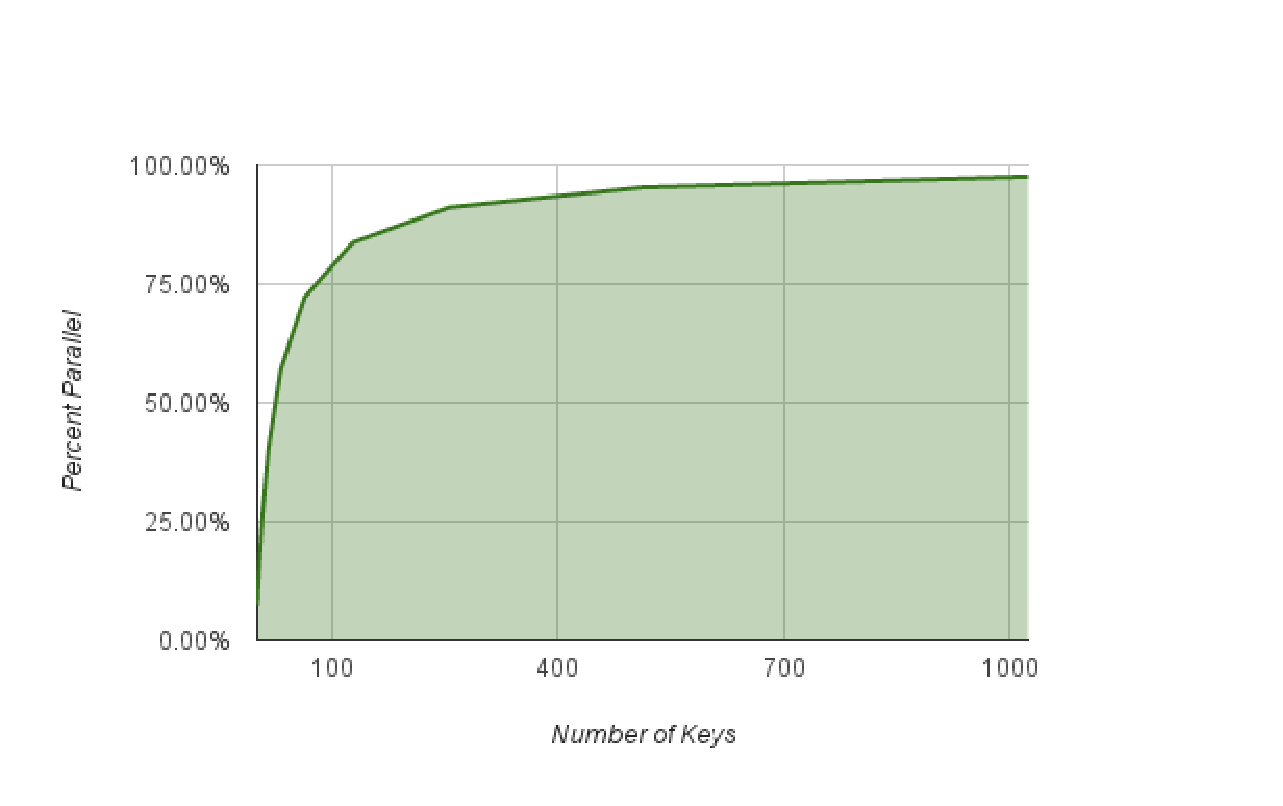
\includegraphics[width=0.75\textwidth]{chart_7}
   \caption{Total percentage of CUDA implementation that is parallel}
   \label{fig:parPercent}
\end{figure}

%%%%%%%%%%%%%%%%%%%%%%%%%%%%%%%%%%%%%%%%%%%%%%%%%%%%%%%%%%%%%%%%%%%%%%%%%%%%%%%%

\section{Problem Description}
\label{sec:probdesc}
The RSA weakness described above demands that each key in a set be 
compared with each other key to determine if a GCD greater than 1 exists for 
any pair. Given a known set of keys, it is not known before processing 
the keys which will be likely to have a GCD greater than 1; therefore, there 
is no way to eliminate comparisons between specific pairs. The natural 
organization to fulfill this requirement is a diagonally-symmetric comparison
matrix of the all keys. Each location in the matrix corresponds to a GCD
comparison between two keys.

%%%%%%%%%%%%%%%%%%%%%%%%%%%%%%%%%%%%%%%%%%%%%%%%%%%%%%%%%%%%%%%%%%%%%%%%%%%%%%%%

\section{Implementation}
\label{sec:impl}

\subsection{Problem Decomposition}
\label{subsec:probdecomp}

Initially, the comparison matrix seems to be an $n^2$ solution. However, the 
diagonal of the matrix created consists of unproductive GCD calculations since 
these entries would compare each key with itself. Furthermore, the matrix is 
symmetrical over the diagonal. Thus, only the comparisons comprising the upper
or lower triangle of the matrix needs to be performed. Specifically, 

\begin{equation}
   \mbox{Total number of GCD compares} = \sum_{i=1}^{k-1} i
   \label{eq:gcd}
\end{equation}

%This reduction in number of overall compares decreases the work 
%performed significantly, shown in Figure~\ref{fig:compvkeys}. 

%\begin{figure}
   %\centering
   %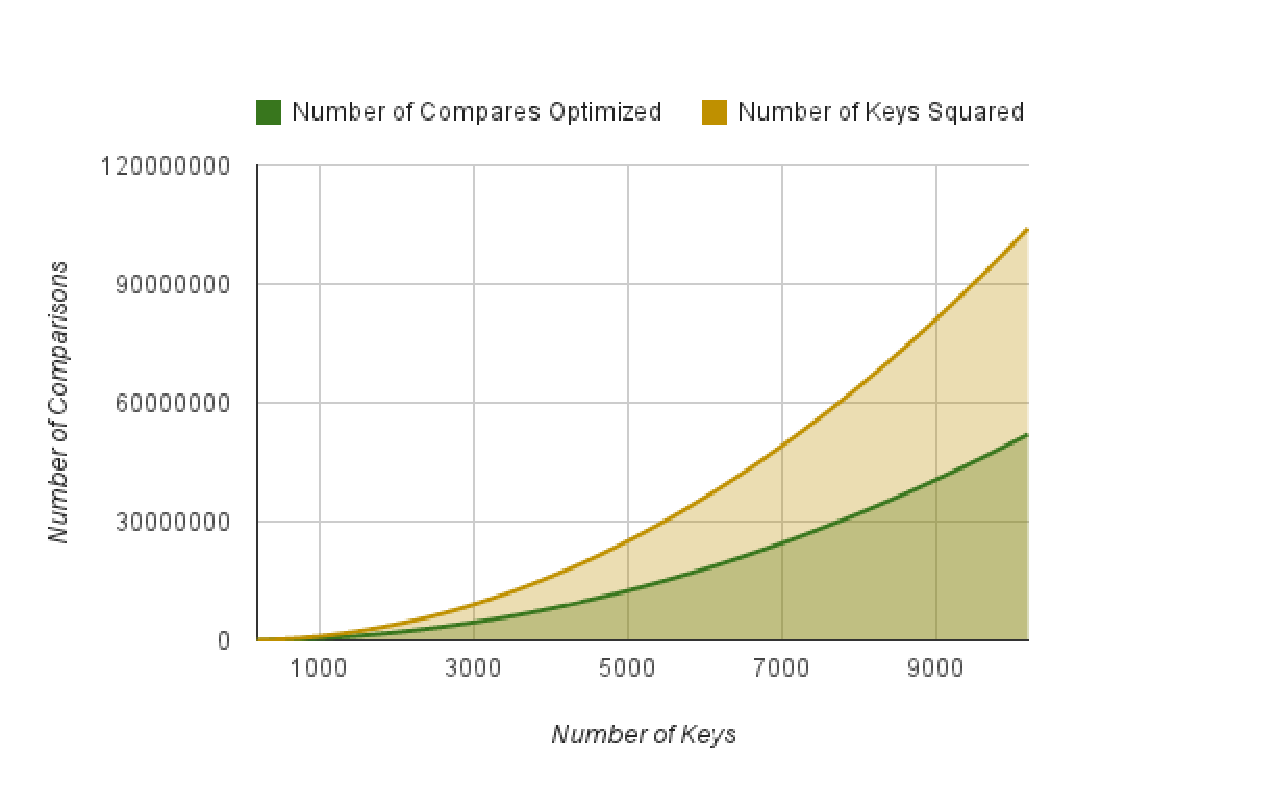
\includegraphics[width=0.75\textwidth]{chart_6}
   %\caption{Number of comparisons needed vs. total number of keys in set}
   %\label{fig:compvkeys}
%\end{figure}

\subsection{Grid Organization}
\label{subsec:gridorg}
One of the most important aspects of any CUDA implementation is the 
organization of the thread and block array to ensure that the architecture is 
appropriately used to its full potential. The threads array in this 
implementation was organized using three dimensions. The $x$ dimension
represented the sectioning of a 1024-bit value into individual 32-bit integers,
of which there are 32. 

\begin{displaymath}
   \frac{1024 \:\mbox{bits per key}}{32 \:\mbox{bits per integer}} = 
   32 \;\mbox{integers per key}
\end{displaymath}

The remaining dimensions, $y$ and $z$, were set to 4, resulting in a block of 
512 threads. This design decision was experimentally determined. See 
$\S$\ref{sec:occupancy} for details about Occupancy optimizations.

\begin{displaymath}
   32 \times 4 \times 4 = 512
\end{displaymath}

The $4\cdot4$ dimensions of the block ensured that each block remained square
for algorithmic symmetry and simplicity. These dimensions, $y$ and $z$,
correspond to how many specific keys within the list of all keys are being
compared per block. Thus, two 1024-bit keys are loaded into each 32-thread
warp, which is then processed simultaneously as a single comparison. The $x$
dimension is chosen for two reasons: 1) so one thread in this dimension would
represent each of the 32-bit integers inside the key and 2) because there are
32 threads in a single warp. Therefore, this thread-array organization ensures
that compares are done using two entire keys (separated into 32 pieces) that
are scheduled to the same warp. This eliminates warp divergence since every
warp is filled and executed with non-overlapping data.

Blocks are arranged in row-major order based on the key comparisons that they 
hold. The formula for the number of blocks, $B$, needed for a vector of keys of 
size $k$ can be seen in Equation~\ref{eq:blocks}.

\begin{equation}
   \sum_{i=1}^{\left\lceil \frac{k}{4} \right\rceil}i = B
   \label{eq:blocks}
\end{equation}

The block limit for a grid in a single dimension is $2^{16} - 1 = 65535$ 
and limits the amount of keys that can be processed to $1444$. To increase 
the number of blocks available for computation, a second grid dimension was 
added. This increases the theoretical maximum number of keys per kernel 
launch as seen in Equation~\ref{eq:maxKeys}.

\begin{equation}
   \begin{split}
   \sum_{i = 1}^{\left\lceil\frac{k}{4}\right\rceil} i & \leq {\left(2^{16} - 
   1\right)}^2\\
   k & \leq 370716\\
   \end{split}
   \label{eq:maxKeys}
\end{equation}

\subsection{XY Coordinate mapping}
\label{subsubsec:xymap}

Due to the work-reduction step taken in Section~\ref{subsec:probdecomp}, a
traditional CUDA 2D block arrangement was not appropriate. The block indices
that would have been advantageous, would have wasted significant resources on
the GPU since we only aim to do half of the work that a full 2D block grid would
provide. Therefore, the block array that was used was essentially one
dimensional. Two dimensions are used (as described in
Section~\ref{subsec:gridorg}) when there are many keys that cannot be allocated
to the GPU with a single CUDA block dimension. However, this second dimension
only adds quantity to the one dimensional list, but the indexes advantages
normally realized by the CUDA block grid could not be used.

To overcome this, an XY coordinate mapping is precomputed and copied to the
GPU. This mapping is a lookup table that converts sequential block numberings
from the upper triangular comparison matrix to x-y coordinate pairs that would
have been accurate in the full comparison matrix. This is a necessary step due
to the process of indexing into the key sets during each comparison and looking
up vulnerable keys once the process is complete.

\subsection{Shared Memory}
\label{subsec:shared}
Shared memory is used to load the necessary keys from global memory. Two 
arrays are created in shared memory, representing the thread-array; both 
three-dimensional, $32\times4\times4$, and have an integer loaded into each 
available space. Each array represents which integers are compared at each
location in the matrix. A side effect of this organization is that each key
will be repeated 4 times within its integer array. However, this greatly
simplifies the GCD algorithm so that only a look-up into each array is needed.
Since shared memory is not the limiting factor for occupancy, it is not a
priority to optimize this aspect of the design and implementation. 

Shared memory is also used within the GCD algorithm, specifically in the 
greater-than-or-equal-to function, and the subtract function. In the 
greater-than-or-equal-to function, a single integer is allocated for each 
comparison within a block. Within the subtract function, shared memory is 
utilized to represent the borrow value for each integer. 

\subsection{Occupancy}
\label{sec:occupancy}
Each SM can be assigned multiple blocks at the same time as long as there are 
enough free registers and shared memory available. The ratio of active warps 
to the maximum number of warps supported by a SM is called \emph{occupancy}. 
On the Fermi architecture, the maximum occupancy is achieved when there are 48 
active warps running on a SM at one time. Greater occupancy gives a SM more
opportunities to schedule warps in a fashion to hide memory accesses, thus,
saturating a SM with many warps is favorable for increasing performance. CUDA
Fermi cards have a total of 32768 registers and 49152 bytes of shared memory
per SM. The implementation here uses 17 registers and 4762 bytes of shared
memory per block and therefore results in a maximum occupancy of 100\%.

By using the CUDA occupancy calculator provided by NVIDIA (cf. 
\cite{nvidia2012gpu}), a plot can be formed comparing the threads per block 
with occupancy. To maintain the same block organization outlined above, the 
block dimensions can be $2\times2, 3\times3, 4\times4, 5\times5$ or 128, 228, 
512, 800 threads, respectively. Table~\ref{tab:occupancy} shows the calculated 
occupancy for these block sizes. A block size of 512 threads was chosen 
because it results in the greatest occupancy and thus the best performance. 

\begin{table}
   \centering
   \begin{tabular}{l|rrrr}
      Threads per block & 128 & 288 & 512 & 800\\
      \hline
              Occupancy & 67\% & 94\% & 100\% & 52\%\\
   \end{tabular}
   \caption{Table giving occupancy for various block dimensions}
   \label{tab:occupancy}
\end{table}

The occupancy calculator was used with the values produced by the scalable
implementation (Section~\ref{subsec:arblength}) on the new Kepler hardware
(Section~\ref{subsubsec:updatedsetup}) to ensure occupancy was not lost. The
choice of 512 threads still produces 100\% occupancy. Some of the values
for the other thread counts in Table~\ref{tab:occupancy} differed, but only
slightly ($< 10\%$).

\subsection{Bit-vector}
\label{subsec:bitvector}
The initial approach was to allocate a large, multi-dimensional array of 
integers that would hold the results of the CUDA GCD calculations. This was 
allocated to the GPU, so each thread could have access as needed; however, 
since the number of results grew at $n^2$, the lack of scalability in this 
approach was quickly apparent. Additionally, performance decreased due to the 
large array that was being sent over the PCIe bus. Memory transfers to 
the GPU are slow, and must be minimized.

After more careful consideration, a new approach was implemented. This approach
has only a single bit allocated per key-compare to mark whether or not the pair 
had a GCD greater than 1. In this way, only 2 bytes (16 bits = 1 bit per 
compare) are necessary per block ($4\times4 = 16$ compares per block), as 
opposed to the previous $16 \cdot 32 \cdot 4 = 2048$ bytes. Despite not having
access to the answer immediately after returning from the kernel calculation,
this approach is more efficient since there is a theoretically small number of
keys that are returned with GCDs greater than 1 (i.e. the flag was set). This
small set is then be re-processed (GCDs calculated) using a different kernel or
using a CPU algorithm. Efficiency is also increased due to the time saved in
memory transfers since there is significantly less memory to transfer after
calling the kernel.

\subsection{Arbitrary Length Key Sets}
\label{subsec:arblength}
PARIS's initial implementation \citep{scharfglass2012breaking} took into
account all the above implementation details; however, it was only able to run
a single CUDA kernel once. Furthermore, comparison runs were constrained by
available memory on a given GPU, so only runs that would fit into the limited
memory could be run successfully.

Decomposing the set of comparisons for an arbitrary number of keys is difficult
due to the $n^2$ nature of the problem. The above-outlined method cannot simply
be repeated for various segments of a key set since this would cause gaps in
the results because comparisons between the segments will be missing. Thus, the
entire comparison matrix is segmented, rather than the key sets, into
manageable sections that are run sequentially.

The full comparison matrix still exists as described above: the upper
triangular elements of a square matrix where each entry is a GCD comparison of
two unique keys from a provided set. This upper triangle is divided into
smaller sections of two types: smaller upper triangles that lie on the
diagonal, and rectangles that reside in the upper portion of the original
matrix (see Figure~\ref{fig:divkeys1}). This partitioning mechanism was chosen
for several reasons, the primary of which is that each of these divisions
result in nearly identical memory requirements and workloads that are passed
to the GPU. 

\begin{figure}
   \centering
   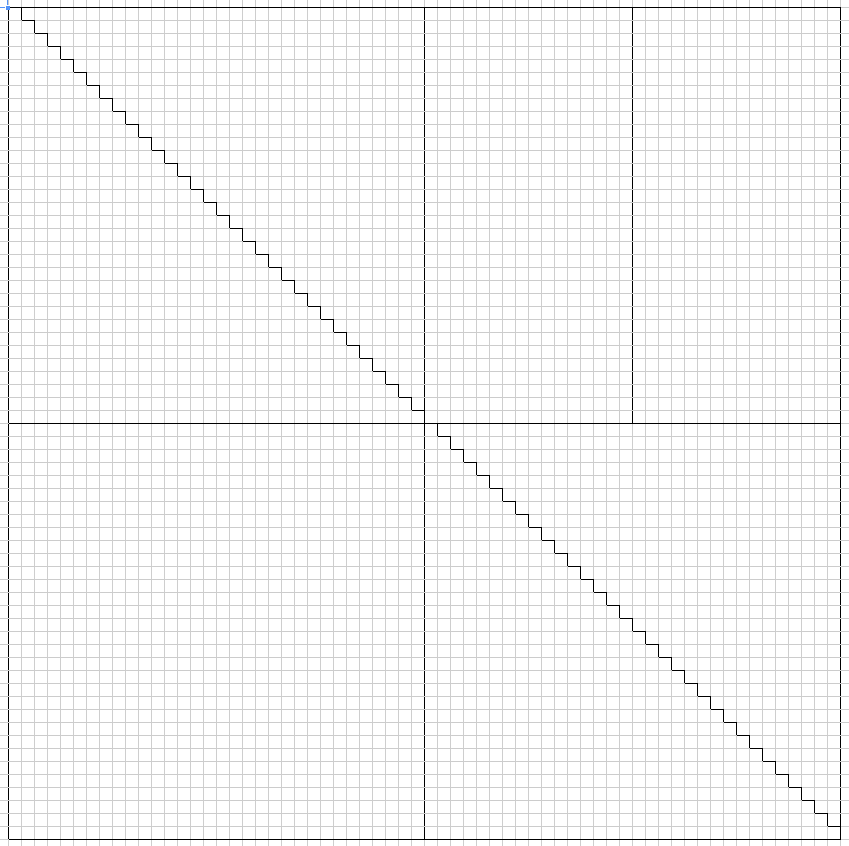
\includegraphics[width=0.7\textwidth]{one_division}
   \caption{A single division of the key matrix}
   \label{fig:divkeys1}
\end{figure}

Depending on the size of the key set provided, it is possible that one of the
divisions shown in Figure~\ref{fig:divkeys1} would still not fit into the GPU
memory. In these cases, a further division is done in a similar way. The upper
triangular segments are partitioned identically as was shown in
Figure~\ref{fig:divkeys1}, and the rectangles are also divided into quadrants. 
Figure~\ref{fig:divkeys3} shows the segments after two additional division
steps. This division process continues until a single segment can fit into the
GPU memory.  

\begin{figure}
   \centering
   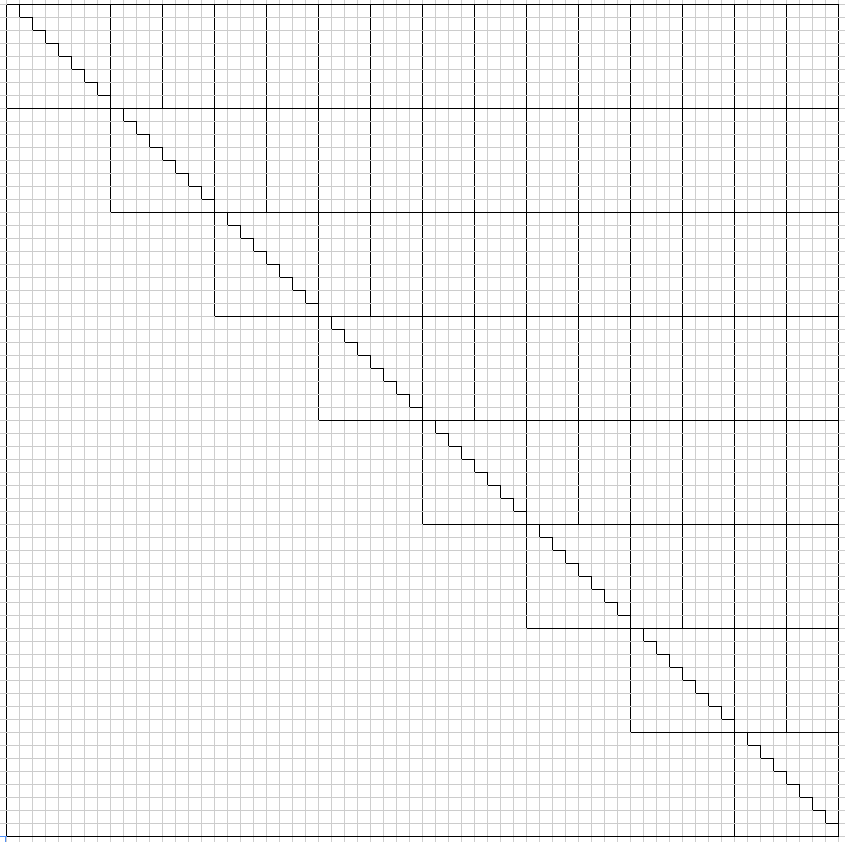
\includegraphics[width=0.7\textwidth]{three_divisions}
   \caption{Three divisions of the key matrix}
   \label{fig:divkeys3}
\end{figure}

To determine when to end the division process, an upper bound for the maximal
number of keys that can fit onto the GPU must be determined. In order to
maximize, we evaluate the memory requirements of each segment. We will use the
following values in our memory calculations:

\begin{displaymath}
   \begin{split}
   T = & \mbox{ the memory needed by an upper triangular segment}\\
       & \mbox{ of key comparisons}\\
   R = & \mbox{ the memory required by a rectangular segment}\\
       & \mbox{ of key comparisons}\\
   y = & \mbox{ number of keys on the y axis being compared}\\
   x = & \mbox{ number of keys on the x axis being compared}\\
   B = & \mbox{ number of CUDA blocks necessary for this key set}\\
   \textrm{KEY\_SIZE} = & \mbox{ the size (in bytes) of a key modulus (128)}\\
   \textrm{XY\_SIZE} = & \mbox{ the size (in bytes) of the x-y coordinate (4)}\\
   \textrm{GCD\_SIZE} = & \mbox{ the size (in bytes) necessary to hold GCD result}\\
               & \mbox{ bits for a single block (2)}
   \end{split}
\end{displaymath}

The triangular portions along the diagonal require three allocations: the set of
keys to compare, the bit-vector to hold the GCD result, and an x-y coordinate
mapping to aid the look-up of keys within the provided set. The x-y coordinate
pair consists of two 16-bit integers (one for $x$, one for $y$), thus the 4
bytes total. The memory calculation is shown in Equation~\ref{eq:trimem}.  

\begin{equation}
   T = y \cdot \textrm{KEY\_SIZE} + B \cdot \textrm{XY\_SIZE} + B \cdot \textrm{GCD\_SIZE}
   \label{eq:trimem}
\end{equation}

\noindent Recall,
\begin{equation}
   B = \sum_{i=1}^{\left\lceil \frac{k}{4} \right\rceil}i
   \tag{\ref{eq:blocks}}
\end{equation}
where $k = $number of keys. We will substitute $k$ for $y$ in the following
calculations since they refer to the same value.  

\noindent Thus,
\begin{equation}
   B = \sum_{i=1}^{\left\lceil \frac{y}{4} \right\rceil}i
   \label{eq:blocksy}
\end{equation}

\noindent We will use the arithmetic sum identity\cite{cohen2011precalculus}
(Equation~\ref{eq:arithident}) to make the
substitution in Equation~\ref{eq:blocksub}.  

\begin{equation}
   \sum_{i=1}^{n}i = \frac{1}{2}n\left(n+1\right)
   \label{eq:arithident}
\end{equation}

\begin{equation}
   B = \frac{1}{2}\left(\frac{y}{4}\right) \left(\frac{y}{4}+1\right)
   \label{eq:blocksub}
\end{equation}

\noindent Continuing Equation~\ref{eq:trimem},
\begin{align}
   T & = y \cdot \textrm{KEY\_SIZE} + B \cdot (\textrm{XY\_SIZE} + \textrm{GCD\_SIZE})\notag\\
   T & = y \cdot 128 + B \cdot (4 + 2)\notag\\
   T & = y \cdot 128 + \left(\frac{1}{2}\left(\frac{y}{4}\right)\left(\frac{y}{4}+1\right)\right) \cdot 6\notag\\
   T & = 128 y + 3 \cdot \frac{y^2}{16} + 3 \cdot \frac{y}{4}\notag\\
   T & = 3 \cdot \frac{y^2}{16} + \frac{515y}{4}
   \label{eq:trimemcomplete}
\end{align}

The rectangular portions also require three allocations: the set of keys in the
$y$ direction, the set of keys in the $x$ direction, and the bit-vector to hold
the GCD result. Equation~\ref{eq:rectmem} outlines the calculation of $R$. Due
to the difference in shape of these GCD results, the number of blocks will not
use the same formula. Instead, the number of blocks is just the area of the
rectangle, shown in Equation~\ref{eq:rectblocks}. Recall, the number of keys is
divided by the dimension of the blocks described in $\S$\ref{subsec:gridorg}.

\begin{equation}
   B' = \frac{y}{4} \cdot \frac{x}{4}
   \label{eq:rectblocks}
\end{equation}

\begin{align}
   R & = y \cdot \textrm{KEY\_SIZE} + x \cdot \textrm{KEY\_SIZE} + B' \cdot \textrm{GCD\_SIZE}\\
   R & = (y + x) \cdot \textrm{KEY\_SIZE} + B' \cdot \textrm{GCD\_SIZE}\notag\\
   R & = (y + x) \cdot 128 + \left(\frac{y}{4} \cdot \frac{x}{4}\right) \cdot 2\notag\\
   \intertext{As mentioned (and as can be seen in Figure~\ref{fig:divkeys1}), $x$ will be half of $y$. Thus,}
   R & = (y + \frac{y}{2}) \cdot 128 + \left(\frac{y}{4} \cdot \frac{\frac{y}{2}}{4}\right) \cdot 2\notag\\
   R & = 128y + 64y + \left(\frac{y}{4} \cdot \frac{y}{4}\right)\notag\\
   R & = \frac{y^2}{16} + 192y
   \label{eq:rectmem}
\end{align}

Comparing $T$ and $R$, we can see that for key sets larger than 506 keys, $T$
is larger. The difference between the functions is increasing, so $T$ will
remain the larger value. Therefore, we can use $T$ as the upper bound for
memory requirements. 

With an equation for evaluating the maximum amount of memory required for a
specified number of keys (Equation~\ref{eq:trimemcomplete}), if a limit on
memory exists, we can determine the maximal number of keys that can fit within
that memory. CUDA offers a function to query the total amount of memory a
device has available (we'll call this $F$). With this value,
Equation~\ref{eq:keycalc} can be used to find the number of keys, $y$.

\begin{align*}
   T & \leq F\\
   3 \cdot \frac{y^2}{16} + \frac{515y}{4} & \leq F\\
   3 \cdot \frac{y^2}{16} + \frac{515y}{4} - F & \leq 0\\
   3 \cdot y^2 + 4\cdot515y- 16 \cdot F & \leq 0\\
   y & = \frac{-b \pm \sqrt{b^2 - 4 \cdot a \cdot c}}{2a}\\
   \text{ with } & a = 3, b = 2060, c = -16F
\end{align*}
\noindent we disregard the `-' since we can't have a negative number of keys
\begin{equation}
   y = \frac{1}{6}\left(-2060 + \sqrt{2060^2 - 192 \cdot F}\right)
   \label{eq:keycalc}
\end{equation}

Equation~\ref{eq:keycalc} is used to find a maximum number of keys for a GPU.
The complete comparison matrix is then segmented as described above until the
size of a segment is smaller than this maximal $y$. The matrix is then iterated
over until all results are computed.

\subsection{Generating the Private Key}
\label{subsec:private}
Once all key comparisons have been processed and the GPU work is complete, the
bit-vector is inspected for ``1"s signifying a vulnerable key was found. When a
``1" is found, the GCD needs to be calculated to generate the private key. As
was shown in Figure~\ref{fig:vuln}, the result of the GCD calculation will be
one of the original prime values. Each of the two moduli that was used in the
GCD calculation is then divided by this value to calculate the other
corresponding primes. The totient ($\phi$) is calculated using the primes.
Finally $d$ is the result of finding the modular multiplicative inverse of
$\phi$ and $e$ (also contained in the public key).

%%%%%%%%%%%%%%%%%%%%%%%%%%%%%%%%%%%%%%%%%%%%%%%%%%%%%%%%%%%%%%%%%%%%%%%%%%%%%%%%

\section{Experimental Setup}
\label{sec:expsetup}

\subsection{Test Machine}
\label{subsec:testmachine}

\subsubsection{Initial Setup}
\label{subsubsec:initsetup}
All performance measurements were made on a single machine with an Intel Xeon 
W3503 dual-core CPU and 4 GB of RAM. This machine has one NVIDIA GeForce
GTX 480 GPU with 480 CUDA cores and 1.5 GB of memory. The CUDA driver 
version present on the machine is 4.2.0, release 302.17, the runtime version is
4.2.9. The CUDA compute capability is version 2.0, and the maximum threads per 
block is 1024, with each warp having 32 threads.

\subsubsection{Updated Setup}
\label{subsubsec:updatedsetup}
An updated hardware configuration was used to generate more current results.
The CPU in the new configuration is an Intel Xeon E5-2650 8-core CPU. It runs at
2.00 GHz with 64 GB of RAM. The NVIDIA Tesla K20Xm GPU was used for testing. It
has 2688 CUDA cores and 6GB of memory. It has compute capability 3.5 and we use
the NVIDIA driver version 304.88. The maximum threads and warp statistics
remain the same.

\subsection{Reference Implementations}
\label{subsec:refimpl}
In order to check the accuracy of the final implementation, as well as to 
provide a point of comparison for benchmarking, two reference implementations 
of this exploit were created. Each was able to use the same format key 
databases (described in $\S$\ref{subsec:testsets}). 

The first implementation was written purely in Python using the open source
PyCrypto cryptography library. This implementation was able to perform the
entire exploit, from finding weak 1024-bit RSA public keys through generating
the discovered private keys. This implementation was not used for performance
comparison as it was dissimilar to the other two implementations. However, it
was used to validate the exploit itself and serve as an algorithm reference.

A sequential version of the binary GCD algorithm was implemented to serve as a 
second validation tool for the CUDA implementation. This version sequentially 
processed the same input as both other implementations and produced output of
the same format. Comparison with this implementation ensured that unexpected
errors did not result merely from processing the data in parallel.

\subsection{Test Sets}
\label{subsec:testsets}
In order to conduct meaningful tests, it was necessary to use an identical 
data set in all tests. To facilitate this, a tool was written in Python to 
generate both regular and intentionally weak RSA key pairs using PyCrypto and
store them in an SQLite3 database. All keys were generated with a 
constant $e$ of 65537, chosen because this was discovered to be a commonly used 
value (cf. \cite{lenstra2012ron}).

The generation process produced a database of RSA key pairs. 
Intentionally weak keys were evenly distributed. 

In order to generate a weak key, this program would generate an initial 
normal RSA key but save the prime used for $p$. For each subsequent bad key, 
$p$ would be replaced with this constant, and $n$ was recalculated. The 
result was that each weak key would have a GCD greater than 1 when 
tested against any other weak key, namely, $p$. 

Using this tool, it was possible to build arbitrarily large test sets with a 
known number of keys exhibiting the weakness. When these databases 
were processed using any of the reference implementations, the 
discovered number of weak keys could be directly compared with the 
number of keys expected to be found. This allowed both repeatable testing to 
measure run time, and a method to validate PARIS was indeed finding GCDs as
expected. 

%%%%%%%%%%%%%%%%%%%%%%%%%%%%%%%%%%%%%%%%%%%%%%%%%%%%%%%%%%%%%%%%%%%%%%%%%%%%%%%%

\section{Results}
\label{sec:results}

\subsection{Initial Implementation}
\label{subsec:initimpl}
The accuracy of the parallel implementation was verified against the 
sequential implementation by using identical test data sets with known 
weak keys. Since both implementations found the same set of compromised keys,
it was validated that these two implementations were internally consistent.
Furthermore, both matched the results of the separate Python reference
implementation: supporting the assertion of accurate functionality. The speedup
of the CUDA implementation (seen in Figure~\ref{fig:speedup}) was calculated by
comparing its run time with that of the sequential implementation. Compare this
with Figure~\ref{fig:parPercent}: this similarity is evidence of the
implementation presented here matching with theoretical expectations.

\begin{figure}
   \centering
   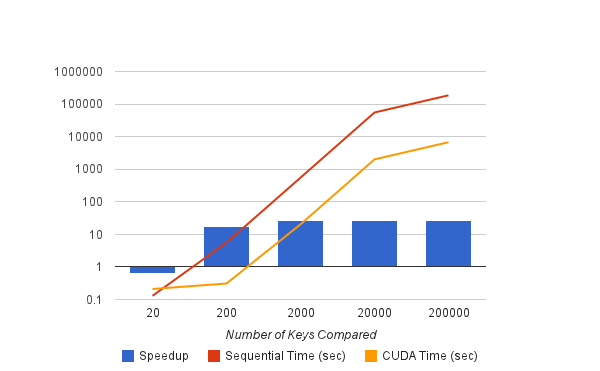
\includegraphics[width=0.75\textwidth]{chart_1}
   \caption{Speedup of CUDA Implementation to Sequential C++ using GTX 480}
   \label{fig:speedup}
\end{figure}

Figure~\ref{fig:speedup} shows that speedup increases dramatically with 
the number of keys until about 2000 comparisons. At this point, the GPU
becomes saturated with enough blocks to fully occupy all of the SMs. Speedup
remains constant at 27.5 for up to 200000 keys. We have no data beyond this
number of keys due to the very long run time of the sequential implementation. 

\begin{table*}
   \centering
   \begin{tabular}{|l|*{5}{r}|}\hline
      Number of Keys        & 20   & 200  & 2000   & 20000    & 200000 \\ \hline
      Sequential Time (sec) & 0.13 & 5.59 & 550.69 & 55121.86 & 185551.91\\
      CUDA Time (sec)       & 0.21 & 0.31 & 20.21  & 2005.09  & 6748.23\\\hline
      \textbf{Speedup}      & 0.6  & 18.0 & 27.2   & 27.5     & 27.5\\\hline
   \end{tabular}
   \caption{Run-times of sequential and CUDA implementations}
   \label{tab:runtimes}
\end{table*}

\subsection{Scalable Implementation}
\label{subsec:scaleimpl}
With the new hardware, PARIS was able to achieve increased speedup of 33.9 as
seen in Figure~\ref{fig:newspeedup}. The set of 20000 keys required just over
200 million GCD calculations, which translates to 4675 comparisons per second.

\begin{figure}
   \centering
   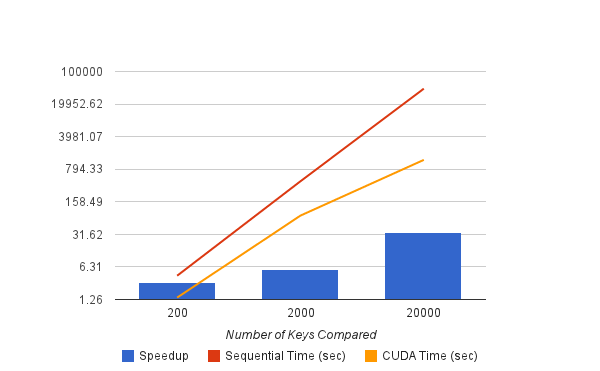
\includegraphics[width=0.75\textwidth]{chart_8}
   \caption{Speedup of CUDA Implementation to Sequential C++ using Tesla K20Xm}
   \label{fig:newspeedup}
\end{figure}

%%%%%%%%%%%%%%%%%%%%%%%%%%%%%%%%%%%%%%%%%%%%%%%%%%%%%%%%%%%%%%%%%%%%%%%%%%%%%%%%

\section{Conclusion}
\label{sec:concl}
A large speedup resulted directly from writing a CUDA 
implementation when compared to the sequential implementation. Many 
more keys are able to be compared in a given amount of time using the CUDA
implementation. 

PARIS is a tool that allows for efficient and complete comparisons of a list of
1024-bit RSA public keys, avoiding repetition and unnecessary work. This tool
allows an increased number of keys to be compared to prior work, in turn
allowing overall execution time to decrease due to the increased parallelism.

PARIS offers significant advantages over other GCD algorithms in CUDA, and
practically applies this for comparison of 1024-bit RSA keys in order to test
for a particular weakness.

%%%%%%%%%%%%%%%%%%%%%%%%%%%%%%%%%%%%%%%%%%%%%%%%%%%%%%%%%%%%%%%%%%%%%%%%%%%%%%%%

\section{Future Work}
\label{sec:future}
To further enhance the throughput of PARIS, asynchronous memory transfers could
be added to the implementation. When combined with multiple kernel launches, a
significant portion of the memory I/O (which is one of the main limiting
factors of performance using the GPU) would be able to be masked by
simultaneously processing the data currently on the GPU while new data is being
copied onto it.

The Kepler architecture introduces new features that may increase the 
performance of this implementation. A feature known as Dynamic Parallelism 
allows a CUDA kernel to launch new kernels from the GPU. This would allow
dynamic allocation of block sizes for different areas of the comparison matrix
and remove idle threads from the kernel. Hyper-Q is a new technology that
manages multiple CUDA kernels from multiple CPU threads. With the current Fermi
architecture, only one CUDA kernel may run on the device at one time. This can
lead to under utilization of the GPU hardware. An approach using multiple CPU
threads, each running their own CUDA kernel, could greatly increase throughput.

We would like to see PARIS maintain a database of keys with unique primes that
it would store after each run. Additionally, it would not only do a full
comparison of all new keys provided to it, but it would use its own key store
to increase the size of the matrix, and lead to a more complete check.

PARIS is still limited to 1024-bit keys due to how well they fit with current
CUDA specifications. While the obvious ideal goal for PARIS would the ability 
to compare keys of arbitrary length, a more reachable goal would be extension
to 2048-bit keys. As mentioned in Section~\ref{subsec:gridorg}, each thread
stores a single 4-byte (32-bit) integer which is a section of the RSA key. CUDA
offers support for a \texttt{long long} type, which would offer 64 bits of
storage space per thread. Leaving the rest of the kernel implementation
identical, it seems as though it might be a straightforward addition that would
allow PARIS to validate a much larger, more relevant (see
Section~\ref{subsec:dataanalysis}) set of keys.

One of our related works \cite{heninger2012mining} mentions an alternative
method of GCD calculations that was able to provide them with significant
speedups. This method focuses on multiplications of large (in our case,
1024-bit) values as opposed to many GCD calculations. It is unclear whether
this would be advantageous given how CUDA handles data and manages its
resources; nonetheless, it would be interesting to investigate algorithmic
changes that could increase our speedup.

%%%%%%%%%%%%%%%%%%%%%%%%%%%%%%%%%%%%%%%%%%%%%%%%%%%%%%%%%%%%%%%%%%%%%%%%%%%%%%%%

\begin{acknowledgements}
We'd like to thank Kerry Scharfglass and Darrin Weng for their contributions
to the original work \cite{scharfglass2012breaking} and fundamental
implementation that formed the basis for the tool.
\end{acknowledgements}

%\appendix
%\section{Appendix}
%\label{app:proofs}
%
%\begin{proof}[Arithmetic Sum Identity]
%\label{proof:asi}
   %\begin{align*}
     %\text{Let } S & = \sum_{i=1}^{n}i\\
      %& = 1 + 2 + \dots + (n - 1) + n\\
      %& = n + (n - 1) + \dots + 2 + 1 && \text{Commutative Property}\\
      %S + S & = (1 + n) + (2 + (n - 1)) + \dots + ((n - 1) + 2) + (n + 1)\\
      %2S & = (n + 1) + (n + 1) + \dots + (n + 1) + (n + 1)\\
      %2S & = n \cdot (n + 1) && \text{$n$ terms in the sum}\\
      %S & = \frac{1}{2} n (n + 1)\\
      %\sum_{i=1}^{n}i & = \frac{1}{2} n (n + 1)\qed
   %\end{align*}
%\end{proof}


% BibTeX users please use one of
\bibliographystyle{spbasic}      % basic style, author-year citations
%\bibliographystyle{spmpsci}      % mathematics and physical sciences
%\bibliographystyle{spphys}       % APS-like style for physics
\bibliography{references}   % name your BibTeX data base

\end{document}
% end of file template.tex

